\chapter{Results}
\autoref{tab:Optical} shows the fractions estimated from the analysis of the BPT diagnostic diagrams for the two samples collecting galaxies selected as BCG and non-BCG. In \autoref{tab:Optical2}, further refinement was implemented by restricting the samples to elements with a signal-to-noise ratio (SNR) greater than 3 and aligning non-BCGs to the same redshift range as BCGs.
In the context of percentages, it is crucial to consider the following points: The additional selection in redshift significantly altered the information captured by the census of both samples. Specifically, within BCGs in Table \autoref{tab:Optical}, the vast majority of species are at least suspected to host an AGN, rather than exhibiting prevalent star-forming characteristics. However, when looking at the same values in Table \autoref{tab:Optical2}, the suspicion becomes almost a certainty. Meanwhile, the BPT-SII analysis goes further, defining the main feedback coming from such AGNs. It is evident in \autoref{tab:Optical} and \autoref{tab:Optical2} that the main population of AGNs shows low ionization ratios.

This change, resulting from the further selection in redshift, also alters the information obtained from non-BCGs census. Initially, the BPT-SII findings indicate that most objects detected as Composite appear to be star-forming galaxies. However, with the subsequent selection in redshift, this assumption becomes less certain, leading to a better subdivision between Liners and SF galaxies.
Finally, to evaluate AGN activity, particularly in the BPT SII diagnostic diagram, the combination of the Seyfert and LINER categories allows a further estimation of the maximum percentage. By comparing the results presented in both tables, BCGs demonstrate an AGN fraction of $(50 \leq P_1 \leq 60)\%$ and $(75 \leq P_2 \leq 90)\%$, according to \autoref{tab:Optical} and \autoref{tab:Optical2} respectively.
In the corresponding context, non-BCGs demonstrate percentages of $(19 \leq P_1 \leq 21)\%$ and $(22 \leq P_2 \leq 55)\%$. This aligns with the findings of Vitale et al. \cite{2012A&A...546A..17V} in the first case and shows a broadened range after the additional selection applied in the second table. In both cases, the conclusion remains unchanged: BCGs are more likely to exhibit AGN activity.
Additional analysis indicates that these fractions remain constant within the redshift range of BCGs (i.e., $0.02 \leq z \leq 0.1$), as illustrated in \autoref{IMG:frac_z}.

Lastly, the analysis dedicated for detecting the BCGs and non-BCGs associated with radio loud emission indicates that BCGs are more likely to host radio luminosity exceeding 5mJy at 1.4 GHz, with a fraction of $12\%$. This value is 20 times higher than the fraction found for the non-BCG subsample of galaxies within the selected regions, as discussed earlier, corresponding to $0.6\%$.

%COSE TENUTE PER SICUREZZA MA MIGLIORATE E DUNQUE DEPRECATE !
\begin{comment}
In \ref{tab:Optical}, detailing the results of the optical analysis, it is observed that BCGs are more likely to host an AGN compared to ordinary galaxies. Percentages obtained for the non-BCG sample are consistent with Vitale et al. \cite{2012A&A...546A..17V}. 

It is noteworthy that the percentages obtained for the non-BCG sample align with the findings of Vitale et al. \cite{2012A&A...546A..17V}. This observation leads to the conclusion that BCGs are more likely to exhibit AGN activity, as discussed in the previous context of percentages.

\end{comment}

\begin{table}[htb]
  \centering
  \begin{tabular}{cccc}
    \hline\hline
    \multicolumn{1}{c}{Diagram} & Classification & non-BCG & BCG \\
    \hline
    [NII]  & AGNs &  $52896 \pm 84$ ($21.1 \pm 0.03$)$\%$ &$161 \pm 5$ ($50.4 \pm 1.6$)$\%$ \\
           & Composites & $55875 \pm 110$ ($22.3 \pm 0.04$)$\%$ & $110 \pm 5$ ($34.5 \pm 1.8$)$\%$ \\
           & SFGs & $141753 \pm 80$ ($56.6 \pm 0.03$)$\%$ &$ 49 \pm 4$ ($15.4 \pm 1.4$)$\%$ \\ 
    \hline
    [SII]  & Seyferts & $13082 \pm 64$ ($6.3 \pm 0.03$)$\%$  &$8 \pm 2$ ($6.5 \pm 1.6$)$\%$\\
           & LINERs & $28396 \pm 80$ ($13.6 \pm 0.04$)$\%$ & $74 \pm 3$ ($53.3 \pm 2.4$)$\%$ \\
           & SFGs &$167826\pm 76 $ ($80.2 \pm 0.04$)$\%$ & $55 \pm 3$ ($40.2 \pm 2.2$)$\%$\\ 
    \hline\hline
  \end{tabular}
  \caption{Results of the classification using BPT diagnostic diagrams, according to the criteria established by Kewley et al. \cite{2006MNRAS.372..961K}. The outcomes are presented in terms of counts per region and as a percentage for each population. }
  \label{tab:Optical}
\end{table}

\begin{table}[htb]
  \centering
  \begin{tabular}{cccc}
    \hline\hline
    \multicolumn{1}{c}{Diagram} & Classification & non-BCG & BCG \\
    \hline
    [NII]  & AGNs & $21.8 \pm 0.1$ $\%$ & $75.4 \pm 2.3$ $\%$ \\
           & Composites & $59.4 \pm 0.1$ $\%$ &  $23.8 \pm 2.3$ $\%$ \\
           & SFGs & $18.8 \pm 0.1$ $\%$ &  $0.73 \pm 0.6$ $\%$ \\ 
    \hline
    [SII]  & Seyferts & $1.7 \pm 0.04$ $\%$  & $0.7 \pm 0.8$ $\%$\\
           & LINERs & $53.44 \pm 0.14$ $\%$  & $89.8 \pm 2$ $\%$\\
           & SFGs &$44.83 \pm 0.1$ $\%$  & $9.5 \pm 2.4$ $\%$\\
    \hline\hline
  \end{tabular}
  \caption{Results of the classification using BPT diagnostic diagrams, following the criteria established by Kewley et al. \cite{2006MNRAS.372..961K}. The samples were additionally refined by requiring a signal-to-noise ratio (SNR) greater than 3 and aligning non-BCGs within the same redshift range as BCGs. The results are presented as percentages for each population. }
  \label{tab:Optical2}
\end{table}

\begin{figure}[t]
  \centering
  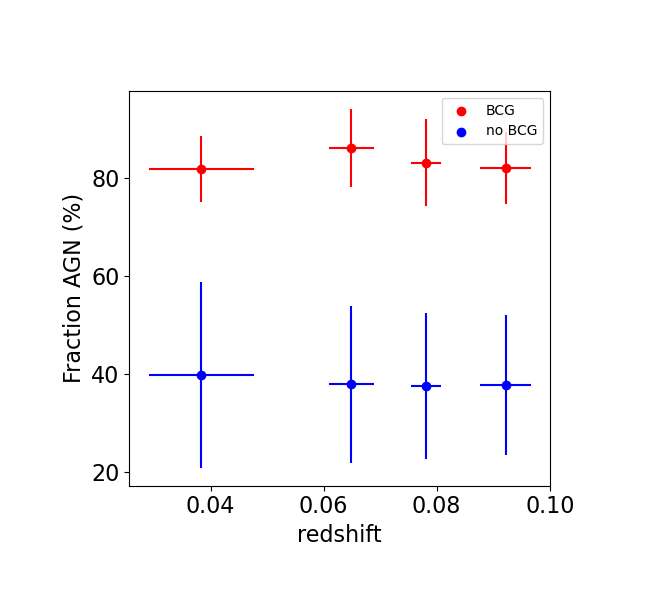
\includegraphics[width=0.85\textwidth]{Fraction_z}
  \caption{Visual representation illustrating the absence of redshift fluctuation in AGN activity percentages, specifically as AGN in the BPT NII diagnostic diagram and as Seyfert + LINER in the BPT SII diagnostic diagram. Redshift bins are uniformly defined to maintain consistent BCG statistics within each bin. The samples underwent further refinement by imposing a signal-to-noise ratio (SNR) threshold greater than 3, and aligning non-BCGs within the identical redshift range as BCGs.}
  \label{IMG:frac_z}
\end{figure}

